% Options for packages loaded elsewhere
\PassOptionsToPackage{unicode}{hyperref}
\PassOptionsToPackage{hyphens}{url}
\PassOptionsToPackage{dvipsnames,svgnames,x11names}{xcolor}
%
\documentclass[
  12pt,
  letterpaper,
  DIV=11,
  numbers=noendperiod]{scrartcl}

\usepackage{amsmath,amssymb}
\usepackage{iftex}
\ifPDFTeX
  \usepackage[T1]{fontenc}
  \usepackage[utf8]{inputenc}
  \usepackage{textcomp} % provide euro and other symbols
\else % if luatex or xetex
  \usepackage{unicode-math}
  \defaultfontfeatures{Scale=MatchLowercase}
  \defaultfontfeatures[\rmfamily]{Ligatures=TeX,Scale=1}
\fi
\usepackage{lmodern}
\ifPDFTeX\else  
    % xetex/luatex font selection
\fi
% Use upquote if available, for straight quotes in verbatim environments
\IfFileExists{upquote.sty}{\usepackage{upquote}}{}
\IfFileExists{microtype.sty}{% use microtype if available
  \usepackage[]{microtype}
  \UseMicrotypeSet[protrusion]{basicmath} % disable protrusion for tt fonts
}{}
\makeatletter
\@ifundefined{KOMAClassName}{% if non-KOMA class
  \IfFileExists{parskip.sty}{%
    \usepackage{parskip}
  }{% else
    \setlength{\parindent}{0pt}
    \setlength{\parskip}{6pt plus 2pt minus 1pt}}
}{% if KOMA class
  \KOMAoptions{parskip=half}}
\makeatother
\usepackage{xcolor}
\usepackage[margin=1in]{geometry}
\setlength{\emergencystretch}{3em} % prevent overfull lines
\setcounter{secnumdepth}{-\maxdimen} % remove section numbering
% Make \paragraph and \subparagraph free-standing
\ifx\paragraph\undefined\else
  \let\oldparagraph\paragraph
  \renewcommand{\paragraph}[1]{\oldparagraph{#1}\mbox{}}
\fi
\ifx\subparagraph\undefined\else
  \let\oldsubparagraph\subparagraph
  \renewcommand{\subparagraph}[1]{\oldsubparagraph{#1}\mbox{}}
\fi


\providecommand{\tightlist}{%
  \setlength{\itemsep}{0pt}\setlength{\parskip}{0pt}}\usepackage{longtable,booktabs,array}
\usepackage{calc} % for calculating minipage widths
% Correct order of tables after \paragraph or \subparagraph
\usepackage{etoolbox}
\makeatletter
\patchcmd\longtable{\par}{\if@noskipsec\mbox{}\fi\par}{}{}
\makeatother
% Allow footnotes in longtable head/foot
\IfFileExists{footnotehyper.sty}{\usepackage{footnotehyper}}{\usepackage{footnote}}
\makesavenoteenv{longtable}
\usepackage{graphicx}
\makeatletter
\def\maxwidth{\ifdim\Gin@nat@width>\linewidth\linewidth\else\Gin@nat@width\fi}
\def\maxheight{\ifdim\Gin@nat@height>\textheight\textheight\else\Gin@nat@height\fi}
\makeatother
% Scale images if necessary, so that they will not overflow the page
% margins by default, and it is still possible to overwrite the defaults
% using explicit options in \includegraphics[width, height, ...]{}
\setkeys{Gin}{width=\maxwidth,height=\maxheight,keepaspectratio}
% Set default figure placement to htbp
\makeatletter
\def\fps@figure{htbp}
\makeatother
\newlength{\cslhangindent}
\setlength{\cslhangindent}{1.5em}
\newlength{\csllabelwidth}
\setlength{\csllabelwidth}{3em}
\newlength{\cslentryspacingunit} % times entry-spacing
\setlength{\cslentryspacingunit}{\parskip}
\newenvironment{CSLReferences}[2] % #1 hanging-ident, #2 entry spacing
 {% don't indent paragraphs
  \setlength{\parindent}{0pt}
  % turn on hanging indent if param 1 is 1
  \ifodd #1
  \let\oldpar\par
  \def\par{\hangindent=\cslhangindent\oldpar}
  \fi
  % set entry spacing
  \setlength{\parskip}{#2\cslentryspacingunit}
 }%
 {}
\usepackage{calc}
\newcommand{\CSLBlock}[1]{#1\hfill\break}
\newcommand{\CSLLeftMargin}[1]{\parbox[t]{\csllabelwidth}{#1}}
\newcommand{\CSLRightInline}[1]{\parbox[t]{\linewidth - \csllabelwidth}{#1}\break}
\newcommand{\CSLIndent}[1]{\hspace{\cslhangindent}#1}

\KOMAoption{captions}{tableheading}
\makeatletter
\@ifpackageloaded{tcolorbox}{}{\usepackage[skins,breakable]{tcolorbox}}
\@ifpackageloaded{fontawesome5}{}{\usepackage{fontawesome5}}
\definecolor{quarto-callout-color}{HTML}{909090}
\definecolor{quarto-callout-note-color}{HTML}{0758E5}
\definecolor{quarto-callout-important-color}{HTML}{CC1914}
\definecolor{quarto-callout-warning-color}{HTML}{EB9113}
\definecolor{quarto-callout-tip-color}{HTML}{00A047}
\definecolor{quarto-callout-caution-color}{HTML}{FC5300}
\definecolor{quarto-callout-color-frame}{HTML}{acacac}
\definecolor{quarto-callout-note-color-frame}{HTML}{4582ec}
\definecolor{quarto-callout-important-color-frame}{HTML}{d9534f}
\definecolor{quarto-callout-warning-color-frame}{HTML}{f0ad4e}
\definecolor{quarto-callout-tip-color-frame}{HTML}{02b875}
\definecolor{quarto-callout-caution-color-frame}{HTML}{fd7e14}
\makeatother
\makeatletter
\makeatother
\makeatletter
\makeatother
\makeatletter
\@ifpackageloaded{caption}{}{\usepackage{caption}}
\AtBeginDocument{%
\ifdefined\contentsname
  \renewcommand*\contentsname{Table of contents}
\else
  \newcommand\contentsname{Table of contents}
\fi
\ifdefined\listfigurename
  \renewcommand*\listfigurename{List of Figures}
\else
  \newcommand\listfigurename{List of Figures}
\fi
\ifdefined\listtablename
  \renewcommand*\listtablename{List of Tables}
\else
  \newcommand\listtablename{List of Tables}
\fi
\ifdefined\figurename
  \renewcommand*\figurename{Figure}
\else
  \newcommand\figurename{Figure}
\fi
\ifdefined\tablename
  \renewcommand*\tablename{Table}
\else
  \newcommand\tablename{Table}
\fi
}
\@ifpackageloaded{float}{}{\usepackage{float}}
\floatstyle{ruled}
\@ifundefined{c@chapter}{\newfloat{codelisting}{h}{lop}}{\newfloat{codelisting}{h}{lop}[chapter]}
\floatname{codelisting}{Listing}
\newcommand*\listoflistings{\listof{codelisting}{List of Listings}}
\makeatother
\makeatletter
\@ifpackageloaded{caption}{}{\usepackage{caption}}
\@ifpackageloaded{subcaption}{}{\usepackage{subcaption}}
\makeatother
\makeatletter
\@ifpackageloaded{tcolorbox}{}{\usepackage[skins,breakable]{tcolorbox}}
\makeatother
\makeatletter
\@ifundefined{shadecolor}{\definecolor{shadecolor}{rgb}{.97, .97, .97}}
\makeatother
\makeatletter
\makeatother
\makeatletter
\makeatother
\ifLuaTeX
  \usepackage{selnolig}  % disable illegal ligatures
\fi
\IfFileExists{bookmark.sty}{\usepackage{bookmark}}{\usepackage{hyperref}}
\IfFileExists{xurl.sty}{\usepackage{xurl}}{} % add URL line breaks if available
\urlstyle{same} % disable monospaced font for URLs
\hypersetup{
  pdftitle={Surprise - They're Different!},
  pdfauthor={Stefani Langehennig, PhD; Zach del Rosario, PhD; Mine Dogucu, PhD},
  colorlinks=true,
  linkcolor={blue},
  filecolor={Maroon},
  citecolor={Blue},
  urlcolor={Blue},
  pdfcreator={LaTeX via pandoc}}

\title{Surprise - They're Different!}
\usepackage{etoolbox}
\makeatletter
\providecommand{\subtitle}[1]{% add subtitle to \maketitle
  \apptocmd{\@title}{\par {\large #1 \par}}{}{}
}
\makeatother
\subtitle{Comparing Frequentist and Bayesian Instructional Approaches}
\author{Stefani Langehennig, PhD \and Zach del Rosario, PhD \and Mine
Dogucu, PhD}
\date{}

\begin{document}
\maketitle
\begin{abstract}
Implementing quantitative methodological techniques is a crucial piece
of public policy and political science instruction. While Frequentists
statistics are most commonly used when teaching quantitative methods in
the social sciences, little research exists on using Bayesian approaches
in the classroom, or how the outcomes from traditional quantitative
approaches differ from a Bayesian approach. We propose an applied
learning activity for students of political science and public policy
that exposes them to Bayesian methods and explores the differences
between this statistical paradigm and more commonly used approaches. We
do this using a structured interrogation of the
\href{https://screeningtool.geoplatform.gov/en/}{The Climate and
Economic Justice Screening Tool} (CEJST) and the epistemological
framings in the 5E model (Elby and Hammer 2010; Duran and Duran 2004).
The activity illustrates the importance of statistical assumptions, and
by extension, the impact that using different quantitative methods has
on real-world outcomes. The goal of the study is to introduce students,
instructors, and practitioners to a new way of using statistics,
equipping them with the tool set and logical processes necessary to
apply either approach as they interrogate social science problems.
\end{abstract}
\ifdefined\Shaded\renewenvironment{Shaded}{\begin{tcolorbox}[boxrule=0pt, frame hidden, breakable, borderline west={3pt}{0pt}{shadecolor}, interior hidden, enhanced, sharp corners]}{\end{tcolorbox}}\fi

\hypertarget{introduction}{%
\subsection{Introduction}\label{introduction}}

Social scientists routinely make use of quantitative methods to
understand the complex world around them. Approaches employed range from
quasi-experimental, spatial diffusion, and econometric techniques, to
methods that are more qualitative in nature. While Bayesian approaches
are not completely missing from political science and public policy (see
Gill and Witko 2013; Fienberg 2011), they are underutilized as a method
taught among social science academics and practitioners. This omission
is for a few reasons. First, scholars and practitioners in government
and public policy spaces often are not exposed to Bayesian methods when
they are taught quantitative techniques (Gill and Witko 2013). Thus, the
lack of familiarity or the ``mindset shift'' required for learning the
methods means Bayesian techniques are not a regular tool in their
toolkit (\textbf{ferrari2022teaching?}). Second, the reliance on
infusing subjective priors into the methodological approach tends to be
questioned by non-statisticians who have received more traditional
Frequentist training in their disciplines (Fienberg 2011; Freedman
1997).

To remedy this, we propose an applied learning activity for students of
public policy and political science that exposes them to Bayesian
methods, focusing on both the theoretical and practical underpinnings of
the approach. The activity explores the differences between Bayesian
approaches and more commonly used statistical techniques to introduce
students, instructors, and practitioners to new and different ways of
using statistics to investigate real-world problems. Through the
application of this activity, these methods will equip different
audiences with the tool set and logical processes necessary to apply
different quantitative approaches when studying political science and
policy problems. More importantly, using this activity in social science
classrooms will encourage students to interrogate and challenge
differences in the assumptions made, and outcomes produced, in the
statistical approaches they are taught.

What follows is an in-depth examination of how teaching different
quantitative methods results in a more robust way of interrogating
political science and public policy problems. We start by reviewing the
research to date on cross-disciplinary approaches to using quantitative
methods, as well as how this influences students' assumptions about
their own learning using the epistemological framings in the 5E Model
(Elby and Hammer 2010; Duran and Duran 2004). Next, we introduce our
applied activity and describe its implementation in the classroom. We
conclude with a discussion on the importance of incorporating Bayesian
statistics into non-statistics classrooms, as well as extensions of the
activity.

\hypertarget{statistical-inference-for-social-scientists}{%
\subsection{Statistical Inference for Social
Scientists}\label{statistical-inference-for-social-scientists}}

Conveying complex concepts and analytical techniques is one of the most
challenging aspects of teaching (Bates and Jenkins 2007). In addition to
distilling topics down to make them accessible to all students,
instructors are frequently tasked with ensuring that the topics learned
in class translate ``out in the wild'' when students enter their
respective professions. This is true in the social sciences and other
non-statistics disciplines, where students are tasked with translating
what they know into evidence-based practices. While the theories
underpinning non-statistics subjects can be challenging to understand,
layering the quantitative methods typically needed to test research
questions on top of these theories can create added challenges. Too
often the methods and theories, alongside the question of usefulness
outside of the academy, make it difficult to link analysis and political
and policy practices together (Connelly et al. 2021).

What is more, students who are not statistics majors frequently become
anxious and tend to avoid quantitative methods unless the methods are
contextualized and the connection between their subject and technical
approach seems clear (Gunn 2017). Nonetheless, quantitative
methods-particularly statistical inference-are a must for social science
students. Most students take at least a one to three class sequence on
quantitative methods as undergraduates. These usually include some form
of research methods, followed by an applied class that teaches
traditional Frequentist statistical inference (for example, Null
Hypothesis Significance Testing (NHST)).

Some political science and public policy scholars have tried to
incorporate Bayesian philosophy and principles into how estimation is
taught among their students. For instance,
(\textbf{ferrari2022teaching?}) proposes implementing a basic four-step
modeling approach that gets students to shift their thinking from
Frequentist to Bayesian. Similarly, Gill and Witko (2013) offer an
accessible introduction to Bayesian analysis for students of public
administration and policy, arguing that understanding the theoretical
differences between the two approaches is critical, and that Bayesian
techniques are more appropriate for the discipline. Wagner and Gill
(2005) make a similar argument, stressing that Bayesian inference is
``better suited'' for answering public policy questions, showcasing
their application on educational outcomes in public schools. Indeed,
they even go so far as to say that the traditional statistical inference
methods taught in public administration and policy programs is
``defective and should be replaced (Wagner and Gill 2005, 5)'' because
they are borrowed from other disciplines and do not necessarily fit
their research challenges. Finally, Luque and Sosa (2023) use a series
of different scenarios to demonstrate ways in which to incorporate
Bayesian methods into real-world social inquiries. They do this by way
of inferential comparisons between Frequentists and Bayesians,
underscoring the differences between the two approaches both
theoretically and in practice.

\hypertarget{activating-epistemological-frames}{%
\subsubsection{Activating Epistemological
Frames}\label{activating-epistemological-frames}}

One of the primary points stressed in the research advocating for
Bayesian inference in non-statistics classrooms is not to simply
introduce another applied tool without much thought; rather, offering
different philosophies and theoretical approaches in addition to the
tool is crucial to employing effective analytical practices. In social
science quantitative methodology teachings, intellectual development
often starts with a ``surface approach'', where students memorize and
repeat facts that inform them, rather than engaging with or reflecting
on the approaches they have learned (Entwistle 1997; Bates and Jenkins
2007). Our goal, in addition to offering a Bayesian learning activity,
is to move beyond the surface approach, empowering students with the
knowledge to choose between different statistical approaches based on
what is productive for the context at hand. This starts with
epistemological framings, or the nature of knowledge and understanding
among students (Elby and Hammer 2010).

At its most basic level, epistemology is concerned with the methods and
theories that help understand knowledge origins and acquisition.
Epistemological framings are created from personal cognitive resources,
such as beliefs, that are activated among individuals conditional on the
context they are in (Elby and Hammer 2010, 3). These cognitive resources
provide a framework with which individuals can form their understanding
of the ``nature of knowledge, knowing, and learning'', and are often
variable and something that the person may not be aware of (Elby and
Hammer 2010, 4). An epistemological frame is when individual resources
that are reinforced by one another are activated and lead to knowledge
stability (Elby and Hammer 2010, 6). These frames are the expectations
that someone brings to different experiences and scenarios, which in
turn influences their actions.

In the context of the classroom, epistemological frames organize
activities in the classroom for students, which in turn affects their
knowledge and learning. Students who can recognize and critique the
assumptions underpinning their analyses (treating them as tentative),
but carry out their analyses respecting those analyses (treating them as
true) will likely be more effective as practicing statisticians in their
discipline. Getting students to recognize the importance of
assumptions---and to practice adopting different assumptions---is a
critical first step in developing these multiple epistemological
framings.

The goal of our activity is to activate students' epistemological frames
by structuring it around the 5E Model proposed by Duran and Duran
(2004). The 5E Model is based on constructivist pedagogies and rests on
the notion of inquiry-based teaching, or having students discover
information on their own without the direct help of instructors (Duran
and Duran 2004; Uno 1999). The 5E model is captured in the following
figure:

\begin{figure}

{\centering 

\begin{figure}[H]

{\centering 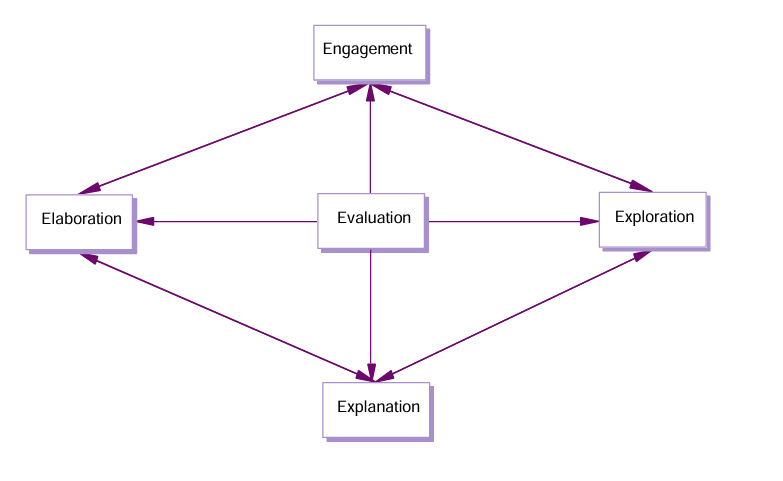
\includegraphics[width=0.75\textwidth,height=\textheight]{01-mpsa-5E.png}

}

\end{figure}

}

\caption{\label{fig-5E}The 5E Instructional Model (as seen in Duran and
Duran (2004), p.52)}

\end{figure}

Each of the E's represent: \emph{Engage}: Get students interested;
\emph{Explore}: Students do self-directed inquiry; \emph{Explain}: Give
students conceptual tools; \emph{Elaborate}: Let students work with the
tools; and \emph{Evaluate}: Assess the learning outcomes. We turn next
to the applied activity, where students compare Frequentist and Bayesian
approaches as applied to a real-world problem.

\hypertarget{sec-applied-activity}{%
\subsection{Applied Activity: Comparing Frequentist \& Bayesian
Approaches}\label{sec-applied-activity}}

To alleviate some of the challenges that come with teaching different
techniques of statistical inference, scholars have compared Frequentist
and Bayesian approaches to one another, highlighting where they are
similar and when they diverge (Samaniego 2010;
\textbf{ferrari2022teaching?}). We do something similar, using a public
policy example to guide our comparison. The activity is focused on a
real dataset, and students follow a structured process to analyze the
dataset and interpret their results. However, different groups receive
different versions of the activity: some receive a Frequentist approach,
while the others receive a Bayesian approach. By carefully crafting the
analyses to reach different conclusions, the aim is to surprise students
with diverging conclusions. The activity concludes with a final
full-group discussion, where the importance of statistical assumptions
are highlighted, completing the comparison of Frequentist and Bayesian
approaches.

The activity learning objectives are three-fold. First, students should
be able to evaluate multiple hypotheses using inferential statistics;
second, students should be able to connect their evaluation of
hypotheses to real-world factors; and third, students should be able to
state the primary statistical assumptions for Frequentist and Bayesian
inference, and understand how they can lead to different conclusions.
These learning objectives stem from our overall learning goal of
engineering a ``classroom controversy'' to motivate students to find
their own understanding of how Frequentist and Bayesian assumptions can
lead to different conclusions (and by extension, real-world
decision-making).

\textbf{Activity Materials}

All materials were created using the programming language \texttt{R} and
can be rendered in .html or .pdf format for use. The materials are
openly available for instructors on our
\href{https://github.com/bayes-bats/tier2-freq-bayes}{GitHub
repository}. Important starter documents include the
\href{https://github.com/bayes-bats/tier2-freq-bayes/blob/main/development/run-of-show.md}{run
of show}, which outlines at a high level the different steps of the
activity, as well as the artifacts used in the activity. Further, the
learning objectives and details of the activity are fleshed out in the
\href{https://github.com/bayes-bats/tier2-freq-bayes/blob/main/development/01-introduction-main.qmd}{introduction
document}. The complete applied activity documents for both the Bayesian
and Frequentist approaches are in the
\href{https://github.com/bayes-bats/tier2-freq-bayes/tree/main/development}{activity
development} folder in the GitHub repository. Instructors can watch a
\href{https://www.youtube.com/watch?v=dwNLcFqQqnE}{video overview} of
the activity on YouTube, and can use the
\href{https://github.com/bayes-bats/tier2-freq-bayes/blob/main/development/Makefile}{Makefile}
available in our repository to compile both student and
instructor-facing artifacts, the latter of which contains solutions and
other notes for running the activity.

\hypertarget{sec-activity-approach}{%
\subsubsection{Activity Approach}\label{sec-activity-approach}}

To implement the activity, there are four steps:

\begin{enumerate}
\def\labelenumi{\arabic{enumi}.}
\tightlist
\item
  Setting the context for the real world problem the class is exploring
\item
  Introducing the motivation for the activity (statistical approaches)
  given the context
\item
  Doing the applied activity
\item
  Closing out the activity
\end{enumerate}

Using the 5E Model, we focus on the applied learning aspects of the
activity, or the application of a statistical approach on current
issues. For example, for \emph{engage} the goal is to motivate students
with current issues around climate and equity. The \emph{explore} stage
is the opportunity in which students get to do self-directed inquiry.
For this activity, that means investigating the real-world dataset
provided to them in small groups. \emph{Explain} gives the students the
conceptual tools they need to understand the different statistical
approaches. Students will learn the basics of assessing and interpreting
a fitted statistical model. For \emph{elaborate}, students get to work
with the tools, meaning they apply the conceptual tools they learned to
the real-world dataset. Finally, \emph{evaluate} involves giving
students the opportunity to reflect on their understanding of the
concepts and application they just did through an instructor-facilitated
class discussion.

Important to this approach is the role of the student. While the
instructor is there to facilitate questions and the general cadence of
the activity, the onus is on students to work through each of the steps
of the activity. This is a fundamental tenant of the 5E model, where
inquiry-based learning is key to students discovering information and
learning.

\hypertarget{sec-prob-context}{%
\paragraph{Problem Context}\label{sec-prob-context}}

We start our activity by introducing
\href{https://screeningtool.geoplatform.gov/en/}{The Climate and
Economic Justice Screening Tool} (CEJST). The CEJST is the result of
President Biden's Executive Order 14008 issued in January 2021. The tool
is used to identify and subsequently help communities disadvantaged by
the burdens stemming from climate change in government social programs.
While the data covers a number of burdens, we focus on the
sustainability aspects of the tool for our activity, including climate
change, energy, and legacy pollution burdens on communities.

We begin with a straightforward explanation of the dataset, situating it
in the contemporary dialogue around climate change. Specifically, we
theorize there may be a relationship between climate change burdens and
minorities residing in Census tracts. By providing them with this
context, we get students to think about possible questions and
hypotheses they may be able to explore using statistical inference.

To dig into the context of our real-world problem further, we also
provide embedded code snippets and output from \texttt{R} of some
high-level exploratory data analysis (EDA) for the students to review
and discuss. We begin by focusing our attention on a few variables of
interest for EDA. We start with the \emph{energy burden percentile},
which captures the percentile of energy cost as well as energy-related
pollution within a census tract, as well as the \emph{percent of
African-American or Black alone}, which captures the percent of
African-American or Black individuals in a census tract.\footnote{While
  we guide our students to the variables we want to explore for this
  implementation of the activity, instructors can modify the activity
  such that students explore the dataset and identify variables of
  interest on their own. If they know how to use statistical software,
  they can also conduct the EDA and analyses in \texttt{R} on their own,
  rather than giving them the completed version as we do here.} After
students have investigated the dataset and have a more thorough
understanding of the problem at hand, the students turn their attention
to the introduction document.

\hypertarget{sec-activity-intro}{%
\paragraph{Activity Introduction}\label{sec-activity-intro}}

This portion of the activity starts with the instructor walking students
through the learning objectives and warm-up questions, which in turn
initiates a group-wide discussion on statistical inference. The
instructor has the students discuss inference at a high level, offering
a more pointed discussion if needed around crafting a research question
and hypotheses. At this point, the instructor turns students to the
simplified
\href{https://github.com/bayes-bats/tier2-freq-bayes/blob/main/development/03-simplified-main.qmd}{critical
differences one-pager} that introduces them to the primary differences
between the Frequentist and Bayesian paradigms. To keep the exercise
manageable, we focus students' attention on \emph{general inference} and
\emph{model summaries}.\footnote{You can access the
  \href{https://github.com/bayes-bats/tier2-freq-bayes/blob/main/development/03-one-pager-main.qmd}{full
  one-pager} that is instructor-facing on the associated GitHub
  repository. In addition to comparing general inference and model
  summaries, it also includes comparisons between fixed variables,
  interpreting probabilities, and model inference.} Table~\ref{tbl-inf}
and Table~\ref{tbl-summ} showcase the critical differences one-pager
containing information on general inference and model summaries:

\hypertarget{tbl-inf}{}
\begin{longtable}[]{@{}
  >{\raggedright\arraybackslash}p{(\columnwidth - 2\tabcolsep) * \real{0.5652}}
  >{\raggedright\arraybackslash}p{(\columnwidth - 2\tabcolsep) * \real{0.4348}}@{}}
\caption{\label{tbl-inf}General Inference}\tabularnewline
\toprule\noalign{}
\begin{minipage}[b]{\linewidth}\raggedright
Frequentist
\end{minipage} & \begin{minipage}[b]{\linewidth}\raggedright
Bayesian
\end{minipage} \\
\midrule\noalign{}
\endfirsthead
\toprule\noalign{}
\begin{minipage}[b]{\linewidth}\raggedright
Frequentist
\end{minipage} & \begin{minipage}[b]{\linewidth}\raggedright
Bayesian
\end{minipage} \\
\midrule\noalign{}
\endhead
\bottomrule\noalign{}
\endlastfoot
Deduction from Pr(data \(|\) H0), by setting \(\alpha\) in advance &
Induction from Pr(\(\theta\) \(|\) data), starting with
Pr(\(\theta\)) \\
Accept H1 if Pr(data \(|\) H0) \textless{} \(\alpha\) & 1−\(\alpha\)\%
of most likely parameter values fall within a 1−\(\alpha\) HPD \\
Accept H0 if Pr(data \(|\) H0) ≥ \(\alpha\) & \\
\end{longtable}

\hypertarget{tbl-summ}{}
\begin{longtable}[]{@{}
  >{\raggedright\arraybackslash}p{(\columnwidth - 2\tabcolsep) * \real{0.5652}}
  >{\raggedright\arraybackslash}p{(\columnwidth - 2\tabcolsep) * \real{0.4348}}@{}}
\caption{\label{tbl-summ}Model Summaries}\tabularnewline
\toprule\noalign{}
\begin{minipage}[b]{\linewidth}\raggedright
Frequentist
\end{minipage} & \begin{minipage}[b]{\linewidth}\raggedright
Bayesian
\end{minipage} \\
\midrule\noalign{}
\endfirsthead
\toprule\noalign{}
\begin{minipage}[b]{\linewidth}\raggedright
Frequentist
\end{minipage} & \begin{minipage}[b]{\linewidth}\raggedright
Bayesian
\end{minipage} \\
\midrule\noalign{}
\endhead
\bottomrule\noalign{}
\endlastfoot
Point estimates and standard errors & Descriptions of the posterior
distribution such as means and quantiles \\
95\% confidence intervals indicating that 19/20 times the interval
covers the true parameter value & Highest posterior density intervals
indicating region of highest posterior probability \\
& 1−\(\alpha\)\% of most likely parameter values fall within a
1−\(\alpha\) HPD \\
\end{longtable}

The introductory discussion of the activity wraps up by introducing the
research question and associated hypothesis the class will test with
their respective statistical approach.\footnote{An extension of the
  activity could have the students develop the research questions and
  hypotheses on their own. Given the activity we implemented is meant to
  span one class period, we provide those for the students.}

\hypertarget{sec-activity-app}{%
\paragraph{Activity Application}\label{sec-activity-app}}

For the activity application, students are assigned a number generated
by a random number generator and put into groups to go through an
applied statistical analysis. There are two versions that are
circulated: the Frequentist analysis and the Bayesian analysis. The
analyses that are given to the students are already completed-they only
receive the output of the analysis with associated questions to help
them think through the different parts of the analysis before they come
to any conclusions.

The data used for each analysis is the exact same for both of the
groups, as is the hypothesis that the students are testing.
Additionally, the students are asked to assess the same conceptual
things, regardless of which statistical approach they receive. They will
use the \emph{general inference} and \emph{model summaries} comparison
discussed in the Section~\ref{sec-activity-intro} to diagnose the
outputs of the models from the analyses.

\textbf{Frequentist Analysis}

Both activities begin with a quick overview of the hypothesis the
students are testing, as well as the different components of a
statistical model. For the Frequentist model, the analysis document
introduces the following model, where \(B\) as the dependent variable
(energy burden percentile), \(P\) is the percent black, \(m\) is the
slope parameter, \(b\) is the intercept parameter, and \(\epsilon\)
captures the error term.

\[{B = m P + b + \epsilon}\] The instructor encourages the class to
think through how to interpret estimates in a linear model using
Frequentist statistics, noting a number of important assumptions along
the way in questions are asked about the model, including that the \(b\)
and \(m\) parameters are fixed but unknown values. This is a natural
place for a number of questions to be asked of the class related to
model summaries and general inference. The questions below illustrate
what the class is asked for understanding model summaries in a
Frequentist model, along with the associated answers:

\begin{tcolorbox}[enhanced jigsaw, arc=.35mm, coltitle=black, leftrule=.75mm, bottomtitle=1mm, colback=white, rightrule=.15mm, colframe=quarto-callout-note-color-frame, toprule=.15mm, left=2mm, opacitybacktitle=0.6, toptitle=1mm, title={Questions for the Class}, colbacktitle=quarto-callout-note-color!10!white, breakable, titlerule=0mm, opacityback=0, bottomrule=.15mm]

\begin{itemize}
\tightlist
\item
  Which scenario gives the largest estimate for the slope?

  \begin{itemize}
  \tightlist
  \item
    Scenario B
  \end{itemize}
\item
  Does the confidence interval for Scenario A include zero? (NB. A
  confidence interval includes zero if Lower \textless{} 0 \textless{}
  Upper.)

  \begin{itemize}
  \tightlist
  \item
    Yes
  \end{itemize}
\item
  Does the confidence interval for Scenario B include zero?

  \begin{itemize}
  \tightlist
  \item
    Yes
  \end{itemize}
\item
  Does the confidence interval for Scenario C include zero?

  \begin{itemize}
  \tightlist
  \item
    No
  \end{itemize}
\item
  If a confidence interval includes zero, this indicates that we cannot
  conclude whether the slope is positive or negative. For which
  scenarios can we not conclude whether the slope is positive or
  negative?

  \begin{itemize}
  \tightlist
  \item
    Scenarios A and B
  \end{itemize}
\end{itemize}

\end{tcolorbox}

After students have revisited the concepts around model summaries and
general inference for the Frequentist linear model, they move to a
predictive model where they are given a number of predicted versus
observed value plots, show below, for the model across three states:
Massachusetts, Colorado, Florida, and the entire sample of data (e.g.,
the U.S.).

\begin{figure}

{\centering 

\begin{figure}[H]

{\centering 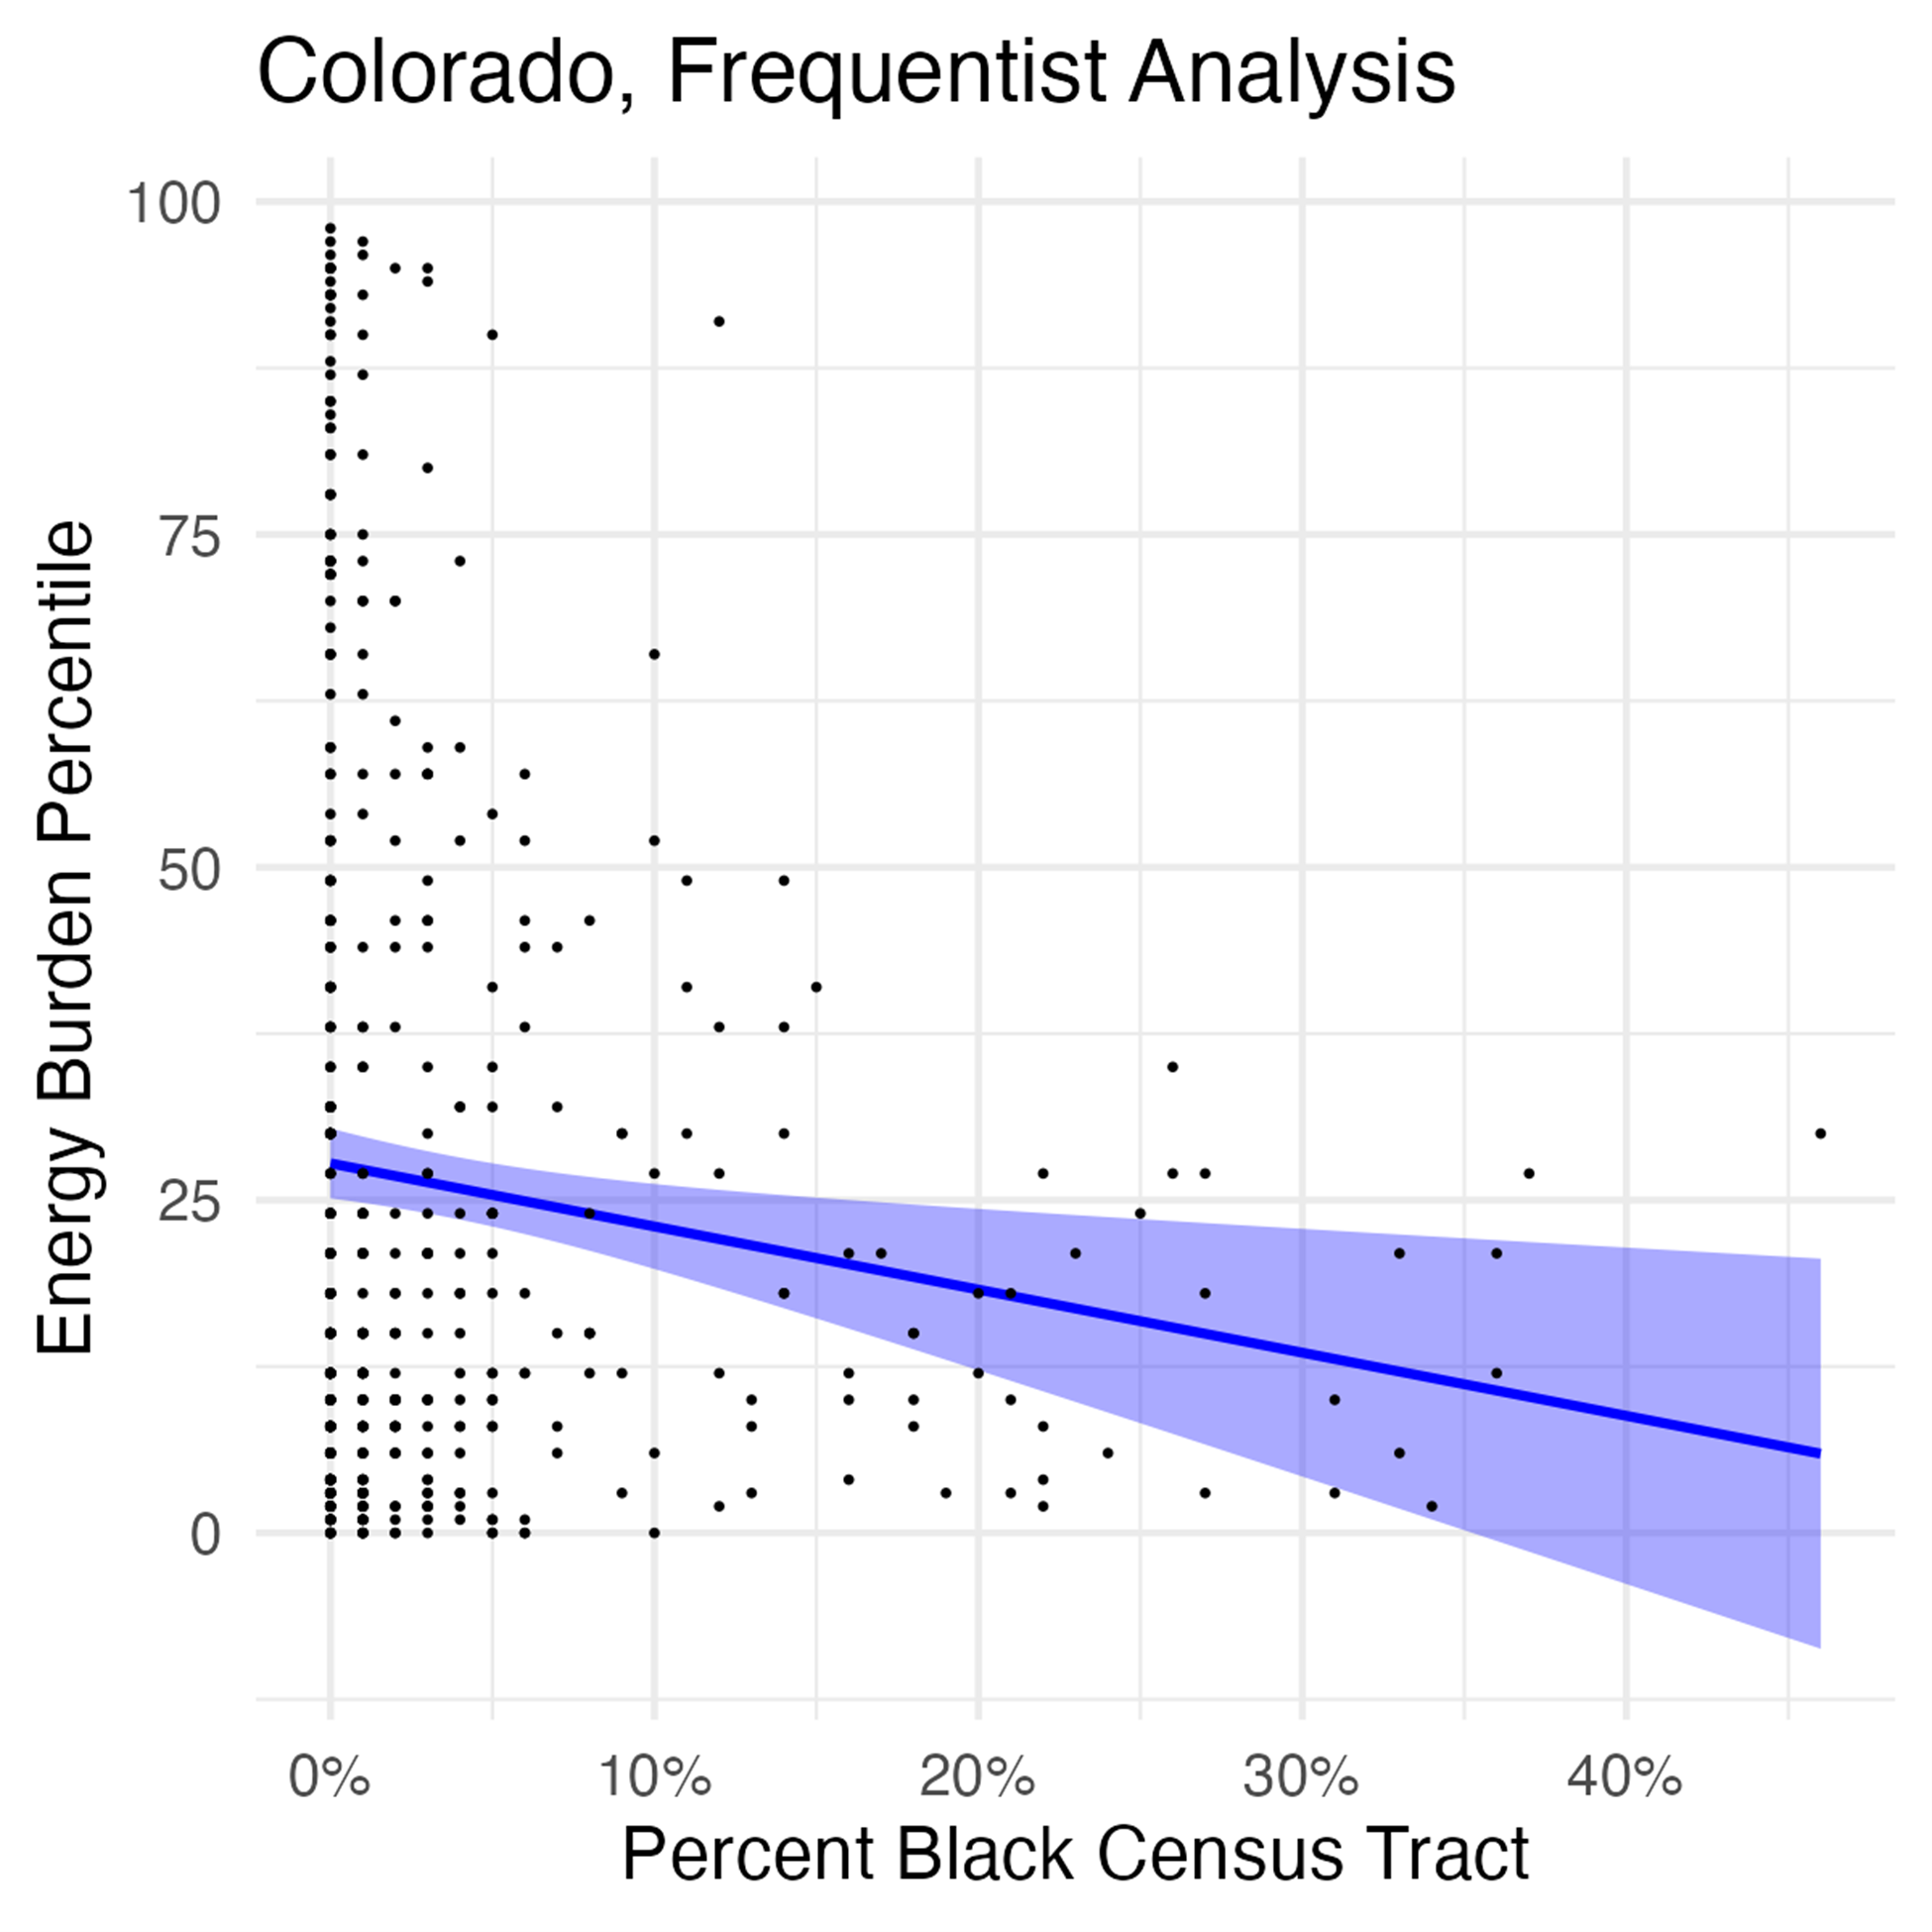
\includegraphics[width=0.5\textwidth,height=\textheight]{01-mpsa-freq-ex1.png}

}

\end{figure}

}

\caption{\label{fig-freq1}Example Trend from Frequentist Analysis}

\end{figure}

Additionally, they are given the intercept and slope estimates, as well
as the confidence intervals for each model.

\begin{figure}

{\centering 

\begin{figure}[H]

{\centering 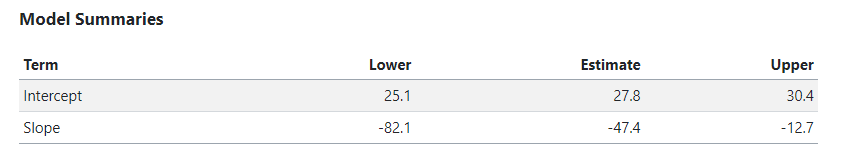
\includegraphics[width=0.7\textwidth,height=\textheight]{01-mpsa-COfreq-ex1.png}

}

\end{figure}

}

\caption{\label{fig-freq2}Example Model Summary from Frequentist
Analysis}

\end{figure}

Once they have seen the results for each of the states and the U.S.,
students are given a set of questions that encourage them to think about
the model results knowing what they do about model summaries and general
inference. At this point, the students are exploring the results of the
model in their respective groups and discussing and answering together
the questions provided to them.

\textbf{Bayesian Analysis}

The cadence of the Bayesian analysis largely mirrors the Frequentist
analysis to begin. Like the Frequentist groups, the Bayesian groups also
revisit the hypothesis they are testing, as well as the different
components of a statistical model, though this time it is a Bayesian
linear model.

\[ B = m P + b + \epsilon \]

where \(B\) is the energy burden percentile, \(P\) is the percent Black,
\(m\) is the slope parameter, \(b\) is the intercept parameter, and
\(\epsilon\) is a \emph{residual} term that represents factors not
accounted for in the model. The residual term is assumed to be normally
distributed \(\epsilon \sim N(0, \sigma^2)\) with an unknown parameter
\(\sigma^2\). All three parameters have a prior distribution, defined
via:

\[
\begin{aligned} m \sim N(\mu_m, \sigma_m^2), \\ b \sim N(\mu_b, \sigma_b^2), \\ \sigma^2 \sim \text{Exponential}(1/s_y), \end{aligned}
\] where \(m, b, \sigma^2\) are independent. The class discusses how to
set the prior through its parameter values
\(\mu_m, \mu_b, \sigma_m^2, \sigma_b^2\) later in the activity. The
instructor also discusses model assumptions for the Bayesian approach at
a high level, stressing one of the fundamental differences between
Frequentists and Bayesians: the intercept \(b\) and slope \(m\)
parameters are treated as random variables with a distribution that
represents our state of knowledge.

As with the Frequentist analysis, there are a number of questions asked
of the class related to model summaries and general inference for the
Bayesians. This time, however, students are shown the posterior
distribution for the slope (\(m\)) and intercept (\(b\)) for a fitted
model using Massachusetts data. The idea here is to get students
thinking about how confident they should be in drawing conclusions from
the model. After they have seen the distributions for these parameters,
they are shown three different posterior distributions for the slope
parameter so they can make sense of the results from the posterior:

\begin{figure}[H]

{\centering 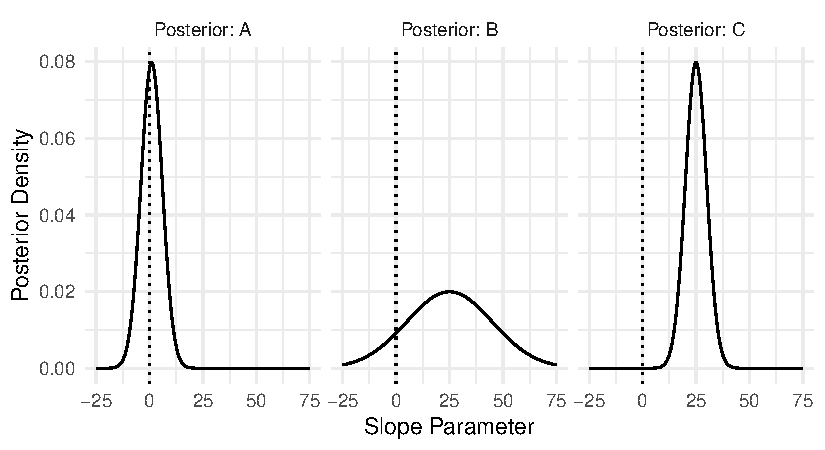
\includegraphics{ps-psci-manuscript_files/figure-pdf/notional-posteriors-1.pdf}

}

\caption{Figure 4: Notational Slope Posteriors for Bayesian Analysis}

\end{figure}

Students are then asked a series of questions, a sample of which are
below, to get them thinking about what the posterior distribution
captures:

\begin{tcolorbox}[enhanced jigsaw, arc=.35mm, coltitle=black, leftrule=.75mm, bottomtitle=1mm, colback=white, rightrule=.15mm, colframe=quarto-callout-note-color-frame, toprule=.15mm, left=2mm, opacitybacktitle=0.6, toptitle=1mm, title={Questions for the Class}, colbacktitle=quarto-callout-note-color!10!white, breakable, titlerule=0mm, opacityback=0, bottomrule=.15mm]

\begin{itemize}
\tightlist
\item
  Roughly, what fraction of \emph{Posterior Distribution A} is greater
  than zero?

  \begin{itemize}
  \tightlist
  \item
    Precisely 57.93\%, so roughly 60\%
  \end{itemize}
\item
  Roughly, what fraction of \emph{Posterior Distribution B} is greater
  than zero?

  \begin{itemize}
  \tightlist
  \item
    Precisely 89.44\%, so roughly 90\%
  \end{itemize}
\item
  Roughly, what fraction of \emph{Posterior Distribution C} is greater
  than zero?

  \begin{itemize}
  \tightlist
  \item
    Essentially 100\%
  \end{itemize}
\item
  Which posterior gives the \emph{highest confidence} (\emph{highest
  probability}) that the slope parameter is positive? How can you tell?

  \begin{itemize}
  \tightlist
  \item
    Posterior C, as the probability is essentially 100\% (as we
    identified above).
  \end{itemize}
\end{itemize}

\end{tcolorbox}

The students have the opportunity to look more closely at the slope
parameter for Massachusetts and discuss it in the context of general
inference. The students should recognize that a positive slope is in
agreement with the hypothesis they are exploring before moving to the
predictive portion of the Bayesian analysis, studying the posterior
predictions.

To further stress the differences between the two approaches, the
activity notes that a prior distribution must also be provided for all
of the components of the model. These priors represent all of our prior
knowledge about the real-world problem the students are trying to solve.
It also ties all of the pieces together, importantly that a fitted
Bayesian model is comprised of the \emph{data + prior = posterior}. The
activity walks the students through hypothetical scenarios where
different prior distributions are used for the slope parameter when
fitting the model with the Massachusetts data. This also shows the
utility of a Bayesian approach when you have limited data, as it allows
us to incorporate prior knowledge, a scenario we use in the activity.

We employ a sequential Bayesian analysis by using the posterior from one
analysis as the prior for a new analysis. We provide the following to
the students in the Bayesian group and have the students pick a state's
prior distribution for the rest of the activity:

\begin{tcolorbox}[enhanced jigsaw, arc=.35mm, coltitle=black, leftrule=.75mm, bottomtitle=1mm, colback=white, rightrule=.15mm, colframe=quarto-callout-note-color-frame, toprule=.15mm, left=2mm, opacitybacktitle=0.6, toptitle=1mm, title={Pick a State}, colbacktitle=quarto-callout-note-color!10!white, breakable, titlerule=0mm, opacityback=0, bottomrule=.15mm]

Study the posteriors above carefully; you will use this as a \emph{prior
distribution} for the slope for the rest of the activity. This means you
will combine \emph{new data} with a \emph{prior distribution} to form a
new \emph{posterior distribution} for the model parameters. The
\emph{prior distribution} should reflect your beliefs about what you
think the slope parameter should be.

Pick \emph{one state for your group}, then come ask the instructor for
your chosen state's packet.

\end{tcolorbox}

\begin{figure}

{\centering 

\begin{figure}[H]

{\centering 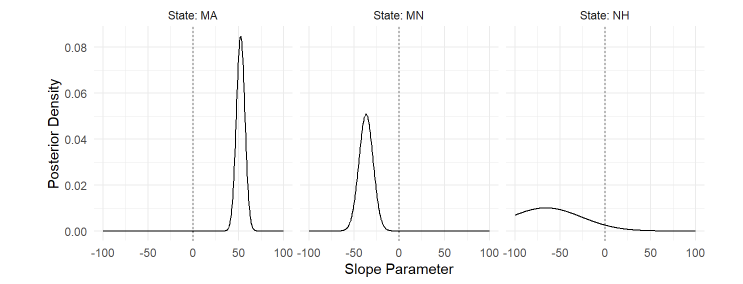
\includegraphics[width=0.75\textwidth,height=\textheight]{01-mpsa-bayesSlope-ex1.png}

}

\end{figure}

}

\caption{\label{fig-slopes2}Example Posterior Choices from Bayesian
Analysis}

\end{figure}

This represents a critical step in the activity for the Bayesians: they
must pick their prior distribution based on their beliefs about what
they think the slope parameter should be. This will subsequently be used
with new data to form a posterior distribution later in the activity.
Each of the results are placed in an envelope, only to be opened once
selected by a group. The following figure represents an example of the
sequential Bayesian analysis used in the full activity that students
will have to choose from and interpret. On the left are the results
showing the fitted lines and slope posteriors for Florida using priors
from Massachusetts, Minnesota, and New Hampshire. On the right are the
results showing the fitted lines and slope posteriors for Colorado, also
using priors from Massachusetts, Minnesota, and New Hampshire.

\begin{figure}[H]

{\centering 

\begin{figure}[H]

{\centering 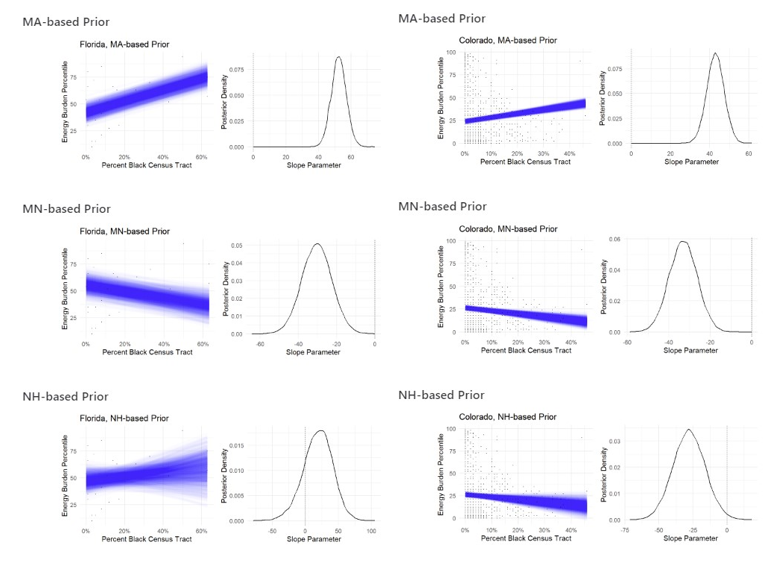
\includegraphics[width=1\textwidth,height=\textheight]{01-mpsa-bayescomp.png}

}

\end{figure}

}

\caption{\label{fig-comparison}Comparison with Different Priors from
Bayesian Analysis}

\end{figure}

\hypertarget{sec-activity-close}{%
\paragraph{Activity Closing}\label{sec-activity-close}}

Once done with the applied portion, groups come back together for a
full-class discussion. In addition to students jotting down any
remaining questions they may have about each of the following questions,
they are posed to the whole class for discussion and are tied to the
learning objectives in Section~\ref{sec-applied-activity}:

\begin{itemize}
\tightlist
\item
  What can we say about our hypothesis?
\item
  How would you answer our research question now that we have analyzed
  the data?
\item
  What can we conclude about the relationship between sustainability and
  disadvantaged communities? What might you recommend from a
  policy-making perspective?
\end{itemize}

We use these questions for a few reasons. The first is so the entire
class can hear the impressions of both groups regarding the statistical
approach used in their analyses. The second is to play into the
``controversy'' or differences between the approaches to further engage
students on the importance of assumptions for statistical conclusions.
The instructor facilitates a debate between the two groups using the
critical differences one-pager discussed in
Section~\ref{sec-activity-intro}. Each group likely thinks their
conclusions are ``correct'' based on their analyses, however it is
important to point out that the controversy cannot be resolved; rather,
the results from our analyses are conditional on the assumptions chosen,
implying that choosing appropriate assumptions is critical to a sound
analysis.

\hypertarget{sec-discussion}{%
\subsection{Discussion}\label{sec-discussion}}

This activity bridges the gap between the common Frequentist approach
oft taught in both undergraduate quantitative methods classes and the
Bayesian paradigm, to which many students have not been exposed. We
believe that non-statistics disciplines, such as political science and
public policy, are an arena with which Bayesian methods can be very
beneficial. To bridge this gap, we use an applied approach with real
world data. While many teaching methods highlight the theoretical
similarities and differences between Frequentists and Bayesians, our
activity moves beyond this by grounding the comparison in a real-data
application. In doing so, we hope to introduce students to a new way of
using statistics, equipping them with the tool set and logical processes
necessary to apply either the Frequentist or Bayesian (or both)
approaches as they see fit.

Our activity uses an active learning approach, rather than relying on
passive lecture. Active learning has been shown to result in superior
learning outcomes for students, particularly those from underrepresented
groups (Freeman et al. 2014). We do this by structuring our activity
around the 5E Model proposed by Duran and Duran (2004), which activates
students' epistemological frames. The 5E Model is based on inquiry-based
teaching, where students \emph{engage, explore, explain, elaborate, and
evaluate} statistical assumptions in an applied setting in order to
promote broader impacts of inferential thinking with respect to
statistics.

The activity described here is intended as a ``minimum viable
activity.'' Future avenues for extending this work include having
students swap groups. Students in this activity only have the chance to
engage deeply with only one of the two paradigms---Frequentist or
Bayesian. A simple extension of the activity would be to have students
re-do their analysis, but switch their approach. This will enable a more
nuanced comparison between Frequentist and Bayesian techniques, which
would add depth to the learning outcomes for students. The second
extension is to create an interactive dashboard. Our initial design for
the activity relies on students' ability to code in \texttt{R}. While
this is feasible in many institutional contexts, it would limit the
portability of the activity to contexts where programming skill is not
so common. Thus, a no-code version of the activity would make it more
accessible. Another extension of the activity would be providing
additional contexts and datasets. Our initial work uses a single context
and dataset for the activity, however this could be re-designed to use a
different context, which would promote the generalizability and impact
of the activity.

Finally, our more speculative research goal---to promote more nuanced
epistemological framings among students---has further potential impacts,
which a survey implemented to the class before and after the activity
may capture. Elby and Hammer (2010) argue that a ``sophisticated''
personal epistemology is actually achieved when one has access to
multiple epistemological framings and can choose to switch between them
based on what is productive for the context at hand. Students who can
recognize and critique the assumptions underpinning their analyses, but
carry out their analyses respecting those analyses, will likely be more
effective as practicing statisticians. Getting students to recognize the
importance of assumptions---and to practice adopting different
assumptions---will be a critical first step in developing these multiple
epistemological framings.

\hypertarget{references}{%
\subsection{References}\label{references}}

\hypertarget{refs}{}
\begin{CSLReferences}{1}{0}
\leavevmode\vadjust pre{\hypertarget{ref-bates2007teaching}{}}%
Bates, Stephen R, and Laura Jenkins. 2007. {``Teaching and Learning
Ontology and Epistemology in Political Science.''} \emph{Politics} 27
(1): 55--63.

\leavevmode\vadjust pre{\hypertarget{ref-connelly2021translating}{}}%
Connelly, Steve, Dave Vanderhoven, Robert Rutherfoord, Liz Richardson,
and Peter Matthews. 2021. {``Translating Research for Policy: The
Importance of Equivalence, Function, and Loyalty.''} \emph{Humanities
and Social Sciences Communications} 8 (1): 1--11.

\leavevmode\vadjust pre{\hypertarget{ref-duran20045e}{}}%
Duran, Lena Ballone, and Emilio Duran. 2004. {``The 5E Instructional
Model: A Learning Cycle Approach for Inquiry-Based Science Teaching.''}
\emph{Science Education Review} 3 (2): 49--58.

\leavevmode\vadjust pre{\hypertarget{ref-elby2010epistemological}{}}%
Elby, Andrew, and David Hammer. 2010. {``Epistemological Resources and
Framing: A Cognitive Framework for Helping Teachers Interpret and
Respond to Their Students' Epistemologies.''} \emph{Personal
Epistemology in the Classroom: Theory, Research, and Implications for
Practice} 4 (1): 409--34.

\leavevmode\vadjust pre{\hypertarget{ref-entwistle1997contrasting}{}}%
Entwistle, Noel. 1997. {``Contrasting Perspectives on Learning.''}
\emph{The Experience of Learning} 2: 3--22.

\leavevmode\vadjust pre{\hypertarget{ref-fienberg2011bayesian}{}}%
Fienberg, Stephen E. 2011. {``Bayesian Models and Methods in Public
Policy and Government Settings.''}

\leavevmode\vadjust pre{\hypertarget{ref-freedman1997some}{}}%
Freedman, David. 1997. {``Some Issues in the Foundation of
Statistics.''} \emph{Topics in the Foundation of Statistics}, 19--39.

\leavevmode\vadjust pre{\hypertarget{ref-freeman2014active}{}}%
Freeman, Scott, Sarah L Eddy, Miles McDonough, Michelle K Smith,
Nnadozie Okoroafor, Hannah Jordt, and Mary Pat Wenderoth. 2014.
{``Active Learning Increases Student Performance in Science,
Engineering, and Mathematics.''} \emph{Proceedings of the National
Academy of Sciences} 111 (23): 8410--15.

\leavevmode\vadjust pre{\hypertarget{ref-gill2013bayesian}{}}%
Gill, Jeff, and Christopher Witko. 2013. {``Bayesian Analytical Methods:
A Methodological Prescription for Public Administration.''}
\emph{Journal of Public Administration Research and Theory} 23 (2):
457--94.

\leavevmode\vadjust pre{\hypertarget{ref-gunn2017embedding}{}}%
Gunn, Andrew. 2017. {``Embedding Quantitative Methods by Stealth in
Political Science: Developing a Pedagogy for Psephology.''}
\emph{Teaching Public Administration} 35 (3): 301--20.

\leavevmode\vadjust pre{\hypertarget{ref-luque2023bayesian}{}}%
Luque, Carolina, and Juan Sosa. 2023. {``Bayesian Analysis for Social
Science Research.''} \emph{arXiv Preprint arXiv:2306.11966}.

\leavevmode\vadjust pre{\hypertarget{ref-samaniego2010comparison}{}}%
Samaniego, Francisco J. 2010. \emph{A Comparison of the Bayesian and
Frequentist Approaches to Estimation}. Vol. 24. Springer.

\leavevmode\vadjust pre{\hypertarget{ref-uno1999handbook}{}}%
Uno, Gordon E. 1999. {``Handbook on Teaching Undergraduate Science
Courses: A Survival Training Manual.''} \emph{(No Title)}.

\leavevmode\vadjust pre{\hypertarget{ref-wagner2005bayesian}{}}%
Wagner, Kevin, and Jeff Gill. 2005. {``Bayesian Inference in Public
Administration Research: Substantive Differences from Somewhat Different
Assumptions.''} \emph{International Journal of Public Administration} 28
(1-2): 5--35.

\end{CSLReferences}



\end{document}
